
In this section we present the mockups of the GUI.

Figure \ref{fig:UserLogin} shows the login page where it's possible to access the registration form for new users.

After login the user will enter the main menu. There are two dfferent access level according to user access level. An end user are not allowed to approved a ticket \ref{fig:MainMenuEndUser} while an authority is privilaged to see and approve a ticket \ref{fig:MainMenuAuthority}.
 by default into the first tab "Report a Violation", see Figure \ref{fig:TakePicture}, where is shown what the camera is recording so the user can start taking the picture of the violation.

For the first time a user logs in some banner can appear showing each function of the app. Also we show on the screen some useful reminders about how the picture to be submitted should be.

After the picture has been taken, the apps shows it as in Figure \ref{fig:pictaken}. A  "brush tool" will appear, which can be used to cover any other plate appearing in the picture, not related to the vehicle being reported.

Figure \ref{fig:FillReport} shows how appears the form where the user has to select the kind of violation he is rporting from a scroll-down list. Each row has an info button, when pressed the GUI will show a verbal description of the violation.

Figure  \ref{fig:ShowStatistic} shows two different statistics that a user can choose.

Figure \ref{fig:MinedOffender} shows the view of the plates which have committed the highest number of violations.

Figure \ref{fig:MinedStreet} shows the view of the heatmap, with a map generated by the external API with the colored overlay which represents the number of violation occurred.

Figure \ref{fig:Ticket} shows the interface only available to Authority Users where are listed all the tickets that are pending for approval. For each ticket all the key informations are shown: picture, location, plate, code of the violation.

 \begin{figure}[H]
		\centering
      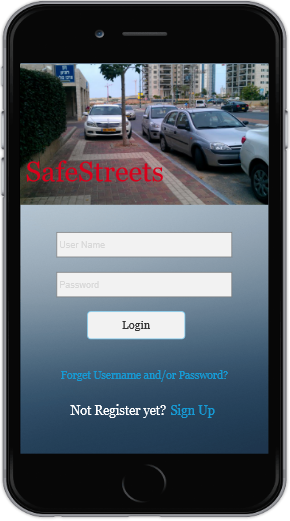
\includegraphics[width=0.5\textwidth]{GUI/UserLogin.png}
      \caption{[GUI] Login screen}   \label{fig:UserLogin}
\end{figure}

\begin{figure}[H]
		\centering
      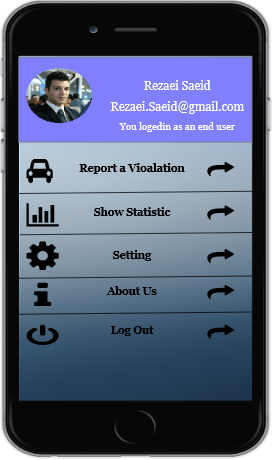
\includegraphics[width=0.5\textwidth]{GUI/MainMenuEndUser.png}
      \caption{[GUI] Main menu for an end user}   \label{fig:MainMenuEndUser}
\end{figure}

\begin{figure}[H]
		\centering
      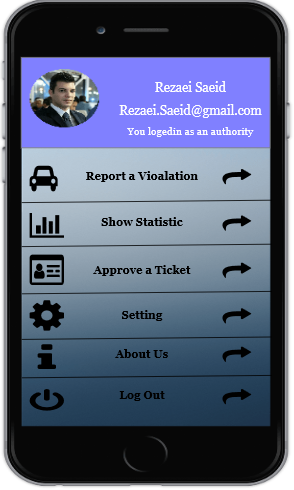
\includegraphics[width=0.5\textwidth]{GUI/MainMenuAuthority.png}
      \caption{[GUI] Main menu for an authority}   \label{fig:MainMenuAuthority}
\end{figure}

\begin{figure}[H]
		\centering
      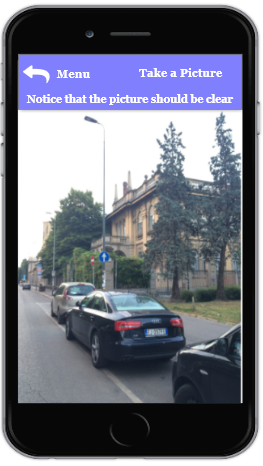
\includegraphics[width=0.5\textwidth]{GUI/TakePicture.png}
      \caption{[GUI] Report | open camera view}   \label{fig:TakePicture}
\end{figure}


\begin{figure}[H]
		\centering
      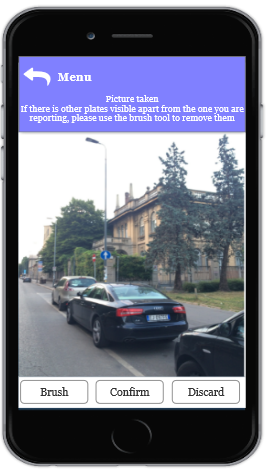
\includegraphics[width=0.5\textwidth]{GUI/pictaken.png}
      \caption{[GUI] Report | picture of violation taken screen}   \label{fig:pictaken}
\end{figure}


\begin{figure}[H]
		\centering
      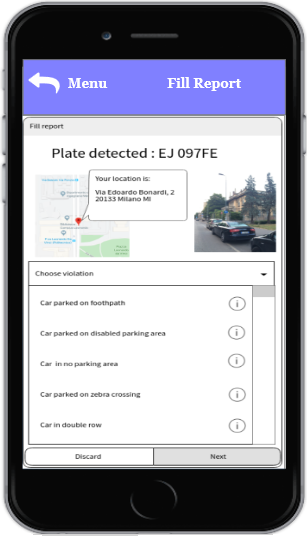
\includegraphics[width=0.5\textwidth]{GUI/FillReport.png}
      \caption{[GUI] Report | violation info form screen}   \label{fig:FillReport}
\end{figure}

///
\begin{figure}[H]
		\centering
      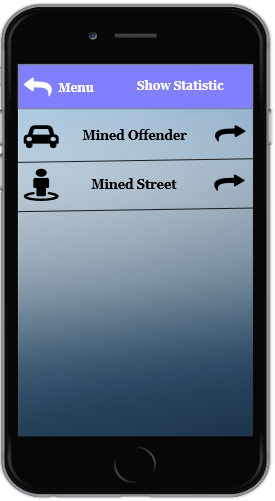
\includegraphics[width=0.5\textwidth]{GUI/ShowStatistic.png}
      \caption{[GUI] Show statistics menu}   \label{fig:ShowStatistic}
\end{figure}

\begin{figure}[H]
		\centering
      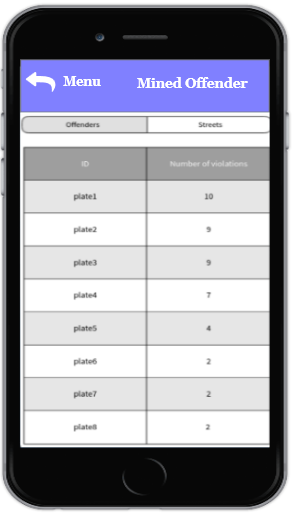
\includegraphics[width=0.5\textwidth]{GUI/MinedOffender.png}
      \caption{[GUI] Explore data screen | offenders}   \label{fig:MinedOffender}
\end{figure}


\begin{figure}[H]
		\centering
      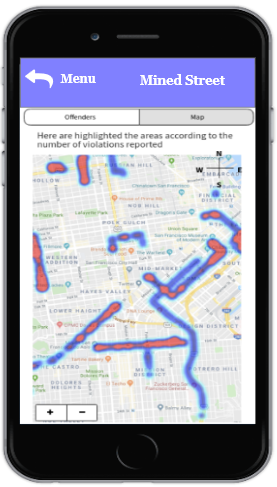
\includegraphics[width=0.5\textwidth]{GUI/MinedStreet.png}
      \caption{[GUI] Explore data | heatmap}   \label{fig:MinedStreet}
\end{figure}


\begin{figure}[H]
		\centering
      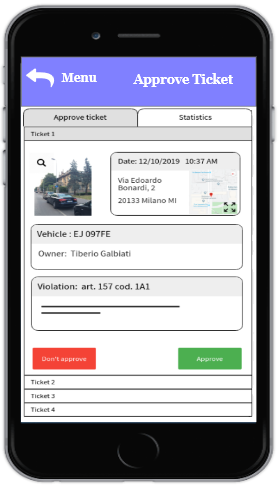
\includegraphics[width=0.5\textwidth]{GUI/Ticket.png}
      \caption{[GUI] Ticket | approval screen}   \label{fig:Ticket}
\end{figure}
